\documentclass[8pt]{beamer}
\geometry{paperwidth=180mm,paperheight=105mm}


\usepackage{amsmath}
\usepackage{wrapfig}
\usepackage{tikz-cd}
\title{Seifert -- Van Kampen Theorem, Applications}
\author{Yahya Tamur}

\begin{document}

  \frame{\titlepage}

  \begin{frame}
    \frametitle{Knots}
    \begin{columns}
      \begin{column}{0.5\textwidth}
        \begin{itemize}
          \item
            A knot is a subset of $\mathbb{R}^3$ homeomorphic to $\mathbb{S}^1$
            (or more generally, any subset of a topological space homeomorphic
            to $\mathbb{S}^n$).
        \end{itemize}

        \begin{center}
        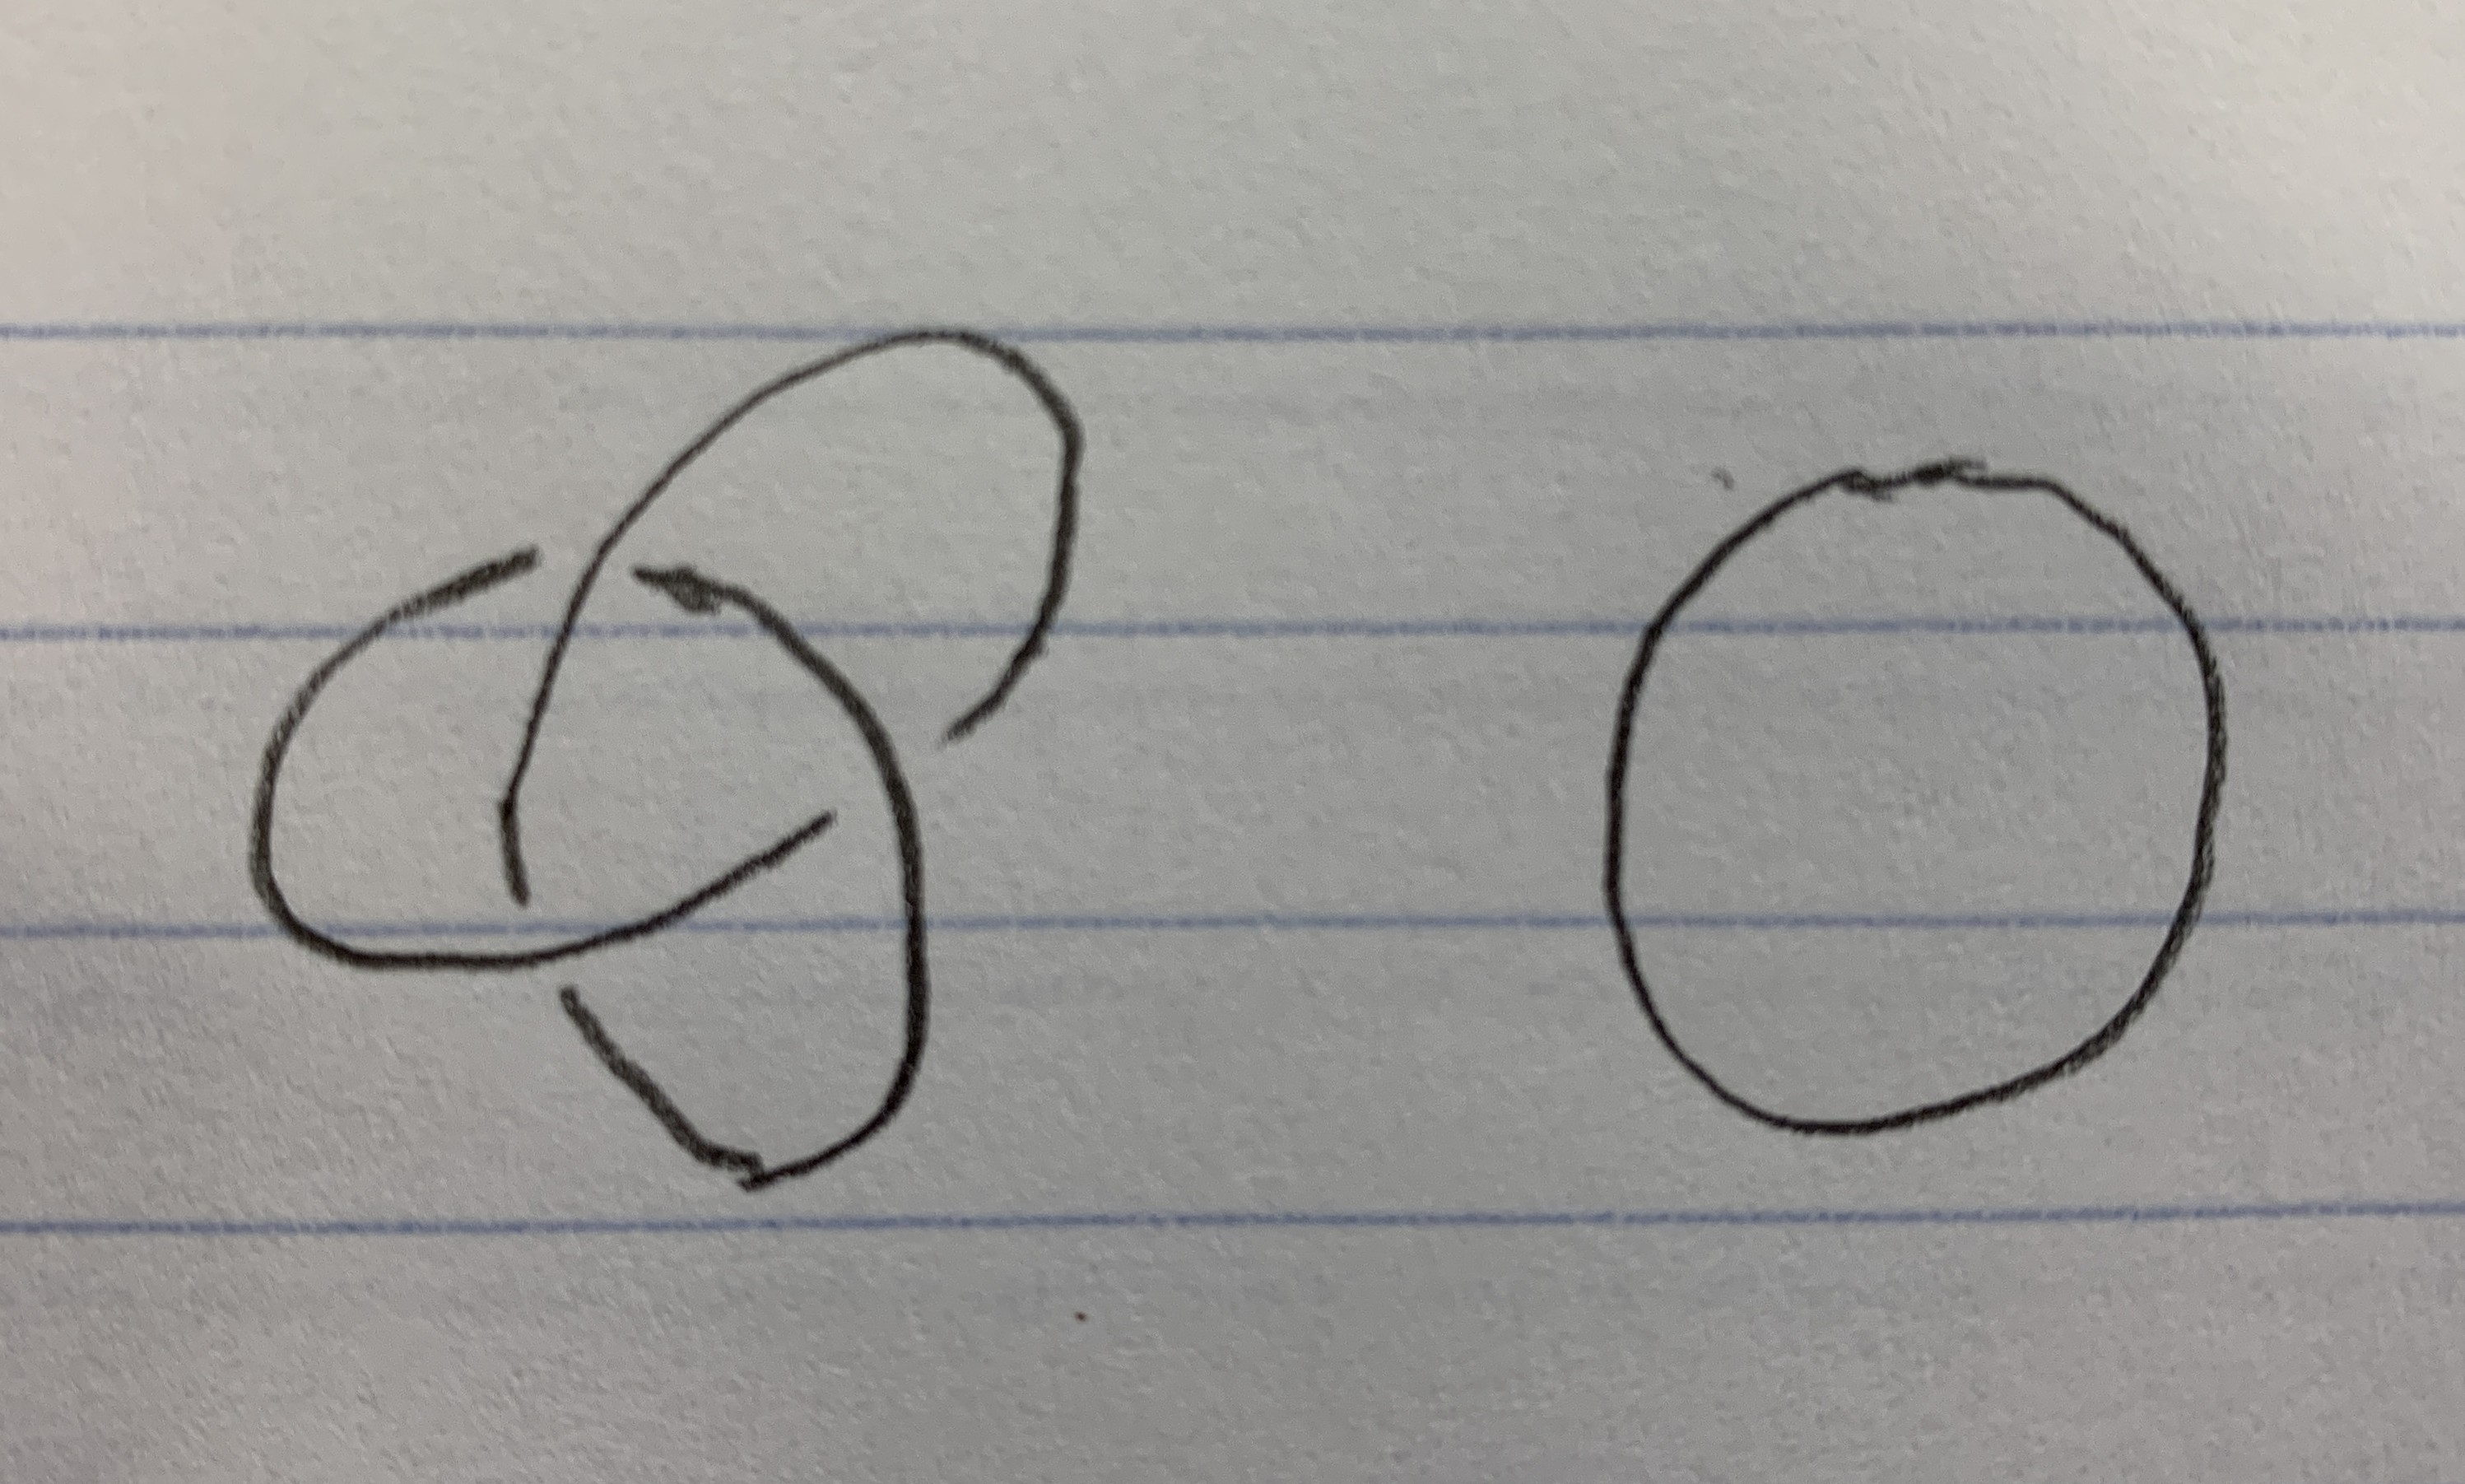
\includegraphics[width=0.7\textwidth]{img/knots.JPG}
        \end{center}

        \begin{itemize}
          \item
            A knot $K$ is equivalent to $K'$ if
            $(K, \mathbb{R}^3)$ is homeomorphic to $(K', \mathbb{R}^3)$

            In other words, there's a homeomorphism
            \[h : \mathbb{R}^3 \rightarrow \mathbb{R}^3 \text{ so that }
            h(K) = K'\]

            Then,
            \[h|_{\mathbb{R}^3-K} : \mathbb{R}^3-K \rightarrow \mathbb{R}^3-K'\]
            is also a homeomorphism,
        \end{itemize}
      \end{column}


      \begin{column}{0.5\textwidth}
        \begin{itemize}
          \item
            ... and its induced homeomorphism from the fundemental groups
            \[\pi_1(\mathbb{R}^3-K) \rightarrow \pi_1(\mathbb{R}^3-K')\]
            is an isomorphism, so those groups are isomorphic.

          \item
            The group $\pi_1(\mathbb{R}^3) - K$ is also called the fundemental
            group of a knot.

          \item
            The main argument we'll be making is, if the fundemental groups of
            two knots aren't isomorphic, then the knots aren't equivalent.

          \item
            Seifert -- Van Kampen's Theorem helps determine the fundemental
            group of $A \cup B$ given the fundemental groups of $A$, $B$, and
            $A \cap B$.

          \item
            In this presentation, we'll be looking at the statement and proof
            of this theorem, and applying it to find the fundemental groups of a
            few knots.
        \end{itemize}
      \end{column}
    \end{columns}
  \end{frame}

  %I literally couldn't explain free groups in a simple way to fit this
  %presentation. like when are two elements the same? when the sequence is
  %different but also you can't have f(s_1)f(s_1)^{-1} next to each other?
  %are we now proving every sequence has a form without those, that form is
  %unique?
  \begin{frame}<0>
    \frametitle{Free Groups}
    \begin{columns}
      \begin{column}[T]{0.5\textwidth}
        \begin{itemize}
          \item To familiarize ourselves with what the theorem looks like,
            here's a more basic definition:
          \item $F$ is the free group of a set $S$ if there's a function
            $f : S \rightarrow F$, and for any group $G$ and function
            $g : S \rightarrow G$, there's a unique homomorphism
            $\sigma : F \rightarrow G$ so that the following commutes:
            \[\begin{tikzcd}[ampersand replacement=\&]
                S \ar[rd, "g"] \ar[r, "f"] \& F \ar[d, "\sigma"]\\
                                                 \& G
              \end{tikzcd}\]
          \item From this definition, we can tell:
          \item For any $s$ in $S$,
            \[\sigma(f(s)) = g(s)\]
          \item Since $\sigma$ is a homomorphism,
            \[\sigma(f(s_1) f(s_2)) = \sigma(f(s_1)) \sigma(f(s_2))
            = g(s_1) g(s_2)\]
            \[\sigma(f(s_1)^{-1}) = g(s_1)^{-1}\]
          \item In fact, this definition well-defines $\sigma$ for any
            $f(s_1)^{a_1} f(s_2)^{a_2} ... f(s_n)^{a_n}$, where
            $a_1, a_2, ... a_n \in \{1,-1\}$
            \[\sigma(f(s_1)^{a_1} f(s_2)^{a_2} ... f(s_n)^{a_n}) =
            g(s_1)^{a_1} g(s_2)^{a_2} ... g(s_n)^{a_n}\]
          \item Since there are no other restrictions on $\sigma$, but $\sigma$
            is unique, $F$ must not have any elements which aren't strings
            \[f(s_1) f(s_2) ... f(s_n)\]
        \end{itemize}
      \end{column}
      \begin{column}[T]{0.5\textwidth}
        \begin{itemize}
          \item For any sequence $\{s_1, s_2, ..., s_n\}$, there's a $G$, $g$
            such that
            \[g(s_1) g(s_2) ... g(s_n) \neq 1\]
            isn't the identity element. Then,
            \[\sigma(f(s_1) f(s_2) ... f(s_n)) \neq 1_G\]
            Since $\sigma$ is a homomorphism,
            \[f(s_1) f(s_2) ... f(s_n) \neq 1_F\]
          \item If $\{s_1, s_2, ... s_n\}$, $\{t_1, t_2 ... t_m\}$ are two
            different sequences, there is a $G$, $g$ so that
            \[g(s_1) g(s_2) ... g(s_n) \neq g(t_1) g(t_2) ... g(t_m)\]
            (Consider the group of finite sequences of elements of $S$ under
            concatenation, $g(s) = \{s\}$. Then,
            \[\sigma(f(s_1) f(s_2) ... f(s_n)) \neq \sigma(f(t_1) f(t_2) ...
            f(t_m))\]
            Then,
            \[f(s_1) f(s_2) ... f(s_n) \neq f(t_1) f(t_2) ... f(t_m)\]
          \item[$\rightarrow$] The elements of $F$ are finite strings
            $f(s_1) f(s_2) ... f(s_n)$ where
            \[f(s_1) f(s_2) ... f(s_n) =
            f(t_1) f(t_2) ... f(t_m)\]
            If and only if $n=m$, $t_1 = s_1$, $t_2 = s_n$, ... $t_m$ = $s_n$.
       
        \end{itemize}
      \end{column}
    \end{columns}
  \end{frame}

  \begin{frame}
    \frametitle{Seifert -- Van Kampen Theorem}
    \begin{columns}
      \begin{column}[T]{0.5\textwidth}
        \begin{itemize}
          \item Let $X$ be a path-connected topological space, $x_0$ be any point
            in $X$. Let $\{U_\lambda\}_{\lambda \in \Lambda}$ be an open cover
            of $X$ so that each $U_\lambda$ contains $x_0$ and the intersection
            of any two elements in the cover is also in the cover.
          \item *here, $\{U_\lambda\}_{\lambda \in \Lambda}$ could be $\{A, B,
            A \cap B\}$*
          \item Let $\psi_\lambda$ be the homomorphism induced by the inclusion
                map $U_\lambda \rightarrow X$.
          \item
            \begin{minipage}[t]{0.5\textwidth}
              \vspace{-5.5mm}
              For $U_\lambda \subseteq U_\mu$, let $\phi_{\lambda\mu}$ be the
              homomorphism induced by the inclusion map $U_\lambda \rightarrow
              U_\mu$. Clearly, the following commutes:
            \end{minipage}%
            \begin{minipage}[t]{0.5\textwidth}
              \centering
              \vspace{-12mm}
                \[\begin{tikzcd}[ampersand replacement=\&]
                  \pi_1(U_\lambda) \ar[rd, "\psi_\lambda"]
                  \ar[r,"\phi_{\lambda\mu}"] \& \pi_1(U_\mu) \ar[d, "\psi_\mu"]
                  \\ \& \pi_1(X)
                  \end{tikzcd}\]
            \end{minipage}
          \item Let $H$ be any group and $\{p_\lambda\}_{\lambda \in \Lambda}$
            be any family of homomorphisms so the following commutes:
            \[\begin{tikzcd}[ampersand replacement=\&]
              \pi_1(U_\lambda) \ar[rd, "p_\lambda"]
              \ar[r,"\phi_{\lambda\mu}"] \& \pi_1(U_\mu) \ar[d, "p_\mu"]\\
                  \& H
              \end{tikzcd}\]
          \item Then, there's a unique $\sigma$ so that the following commutes:
            \[\begin{tikzcd}[ampersand replacement=\&]
                \pi_1(U_\lambda) \ar[rd, "p_\lambda"] \ar[r, "\psi_\lambda"] \&
                \pi_1(X) \ar[d, "\sigma"] \\
                  \& H
              \end{tikzcd}\]
        \end{itemize}
      \end{column}
      \begin{column}[T]{0.5\textwidth}
        From this definition, we can tell:
        \begin{itemize}
          \item If $\alpha \in \pi_1(U_\lambda)$, $\sigma(\psi_\lambda(\alpha)) = p_\lambda(\alpha)$
          \item If $\alpha \in \pi_1(U_\lambda)$, $\beta \in \pi_1(U_\mu)$,
            \[\sigma(\psi_\lambda(\alpha)\psi_\mu(\beta)) =
            \sigma(\psi_\lambda(\alpha))\sigma(\psi_\mu(\beta)) =
            p_\lambda(\alpha)p_\mu(\beta)\]
          \item For $\{\alpha_i\}_{i=1}^n$ so that $\alpha_i \in U_{\lambda_i}$,
            \[\sigma(\psi_{\lambda_1}(\alpha_1)\psi_{\lambda_2}(\alpha_1) ...
            \psi_{\lambda_n}(\alpha_n)) = p_{\lambda_1}(\alpha_1)p_{\lambda_2}(
            \alpha_2) ... p_{\lambda_n}(\alpha_n)\]
          \item We need to prove that $\sigma$ is well defined, In other words,
            if
            \[\psi_{\lambda_1}(\alpha_1) \psi_{\lambda_2}(\alpha_2) ...
              \psi_{\lambda_n}(\alpha_n) \sim \psi_{\mu_1}(\beta_1)
              \psi_{\mu_2}(\alpha_2) ... \psi_{\mu_m}(\mu_m)\]
            Then, $\sigma(\psi_{\lambda_1}(\alpha_1) ...
              \psi_{\lambda_n}(\alpha_n)) \sim \sigma(\psi_{\mu_1}(\beta_1) ...
              \psi_{\mu_m}(\mu_m))$
 
            So, \quad \quad \ \ $p_{\lambda_1}(\alpha_1) ... p_{\lambda_n}(\alpha_n)
              \sim p_{\mu_1}(\beta_1) ... p_{\mu_m}(\beta_m)$
          \item Since this is all the restrictions on $\sigma$, but $\sigma$ is
            unique, $\pi_1(X)$ must not have any elements which aren't in the
            form
              \[\psi_{\lambda_1}(\alpha_1) \psi_{\lambda_2}(\alpha_2) ...
              \psi_{\lambda_n}(\alpha_n)\]
            We also need to prove this.
          \item We'll also look at when two elements of $\pi_1(X)$ are equal and
            when they're different.
          \item But hopefully it makes sense how this theorem determines
            $\pi_1(X)$!
        \end{itemize}
      \end{column}
    \end{columns}
  \end{frame}
  \begin{frame}
    \frametitle{Seifert -- Van Kampen Theorem Proof -- Part 1}
    \begin{columns}
      \begin{column}[T]{0.5\textwidth}
        \begin{itemize}
          \item To Prove: Every element of $a$ $\pi_1(X)$ can be expressed as
            \[a = \psi_{\lambda_1}(\alpha_1)\psi_{\lambda_2}(\alpha_2) ...
              \psi_{\lambda_n}(\alpha_n)\]
            for $\lambda_i \in \Lambda, \alpha_i \in U_{\lambda_i}$.
          \item We will use:

            Lebesgue's Number Lemma: Every open cover of a compact metric space
            has a $\delta$ so that any subset of the metric space with diameter
            less than $\delta$ is contained in a single element of the cover.
            $\delta$ is called the Lebesgue number of the cover.
          \item For any $a \in \pi_1(X)$, find a path $f : [0,1] \rightarrow X$
            so that $a = [f]_{\pi_1(X)}$.
          \item $\{f^{-1}(U_\lambda)\}_{\lambda
            \in \Lambda}$ is a cover of the compact metric space $[0,1]$. It
            has a Lebesgue number $\delta$.
          \item Find $n$ so $\frac{1}{n} < \delta$, divide $[0,1]$ into
            subintervals $[0,\frac{1}{n}]$, $[\frac{1}{n}, \frac{2}{n}]$, ...,
            $[\frac{n-1}{n},1]$. Each has diameter less than $\delta$, so
            $[\frac{i}{n}, \frac{i+1}{n}] \in f^{-1}(U_{\lambda_i})$ for some
            $\lambda_i$, and $f([\frac{i}{n}, \frac{i+1}{n}]) \in U_{\lambda_i}$.
          \item Let $f_i$ be $f$ from $f(\frac{i-1}{n})$ to $f(\frac{i}{n})$. So,
              \[f \sim f_1 f_2 f_3 ... f_n\]
          \item $f(\frac{i}{n}) \in U_{\lambda_i}, U_{\lambda{i+1}}$. Since
            $U_{\lambda_i} \cap U_{\lambda_{i+1}} \in \{U_\lambda\}_{\lambda
            \in \Lambda}$, and all elements of $\{U_\lambda\}_{\lambda \in
            \Lambda}$ are path connected and include $x_0$, there's a path $k_i$
            from $f(\frac{i}{n})$ to $x_0$ contained in $U_{\lambda_i} \cap
            U_{\lambda_{i+1}}$.

        \end{itemize}
      \end{column}
      \begin{column}[T]{0.5\textwidth}

        \begin{center}
          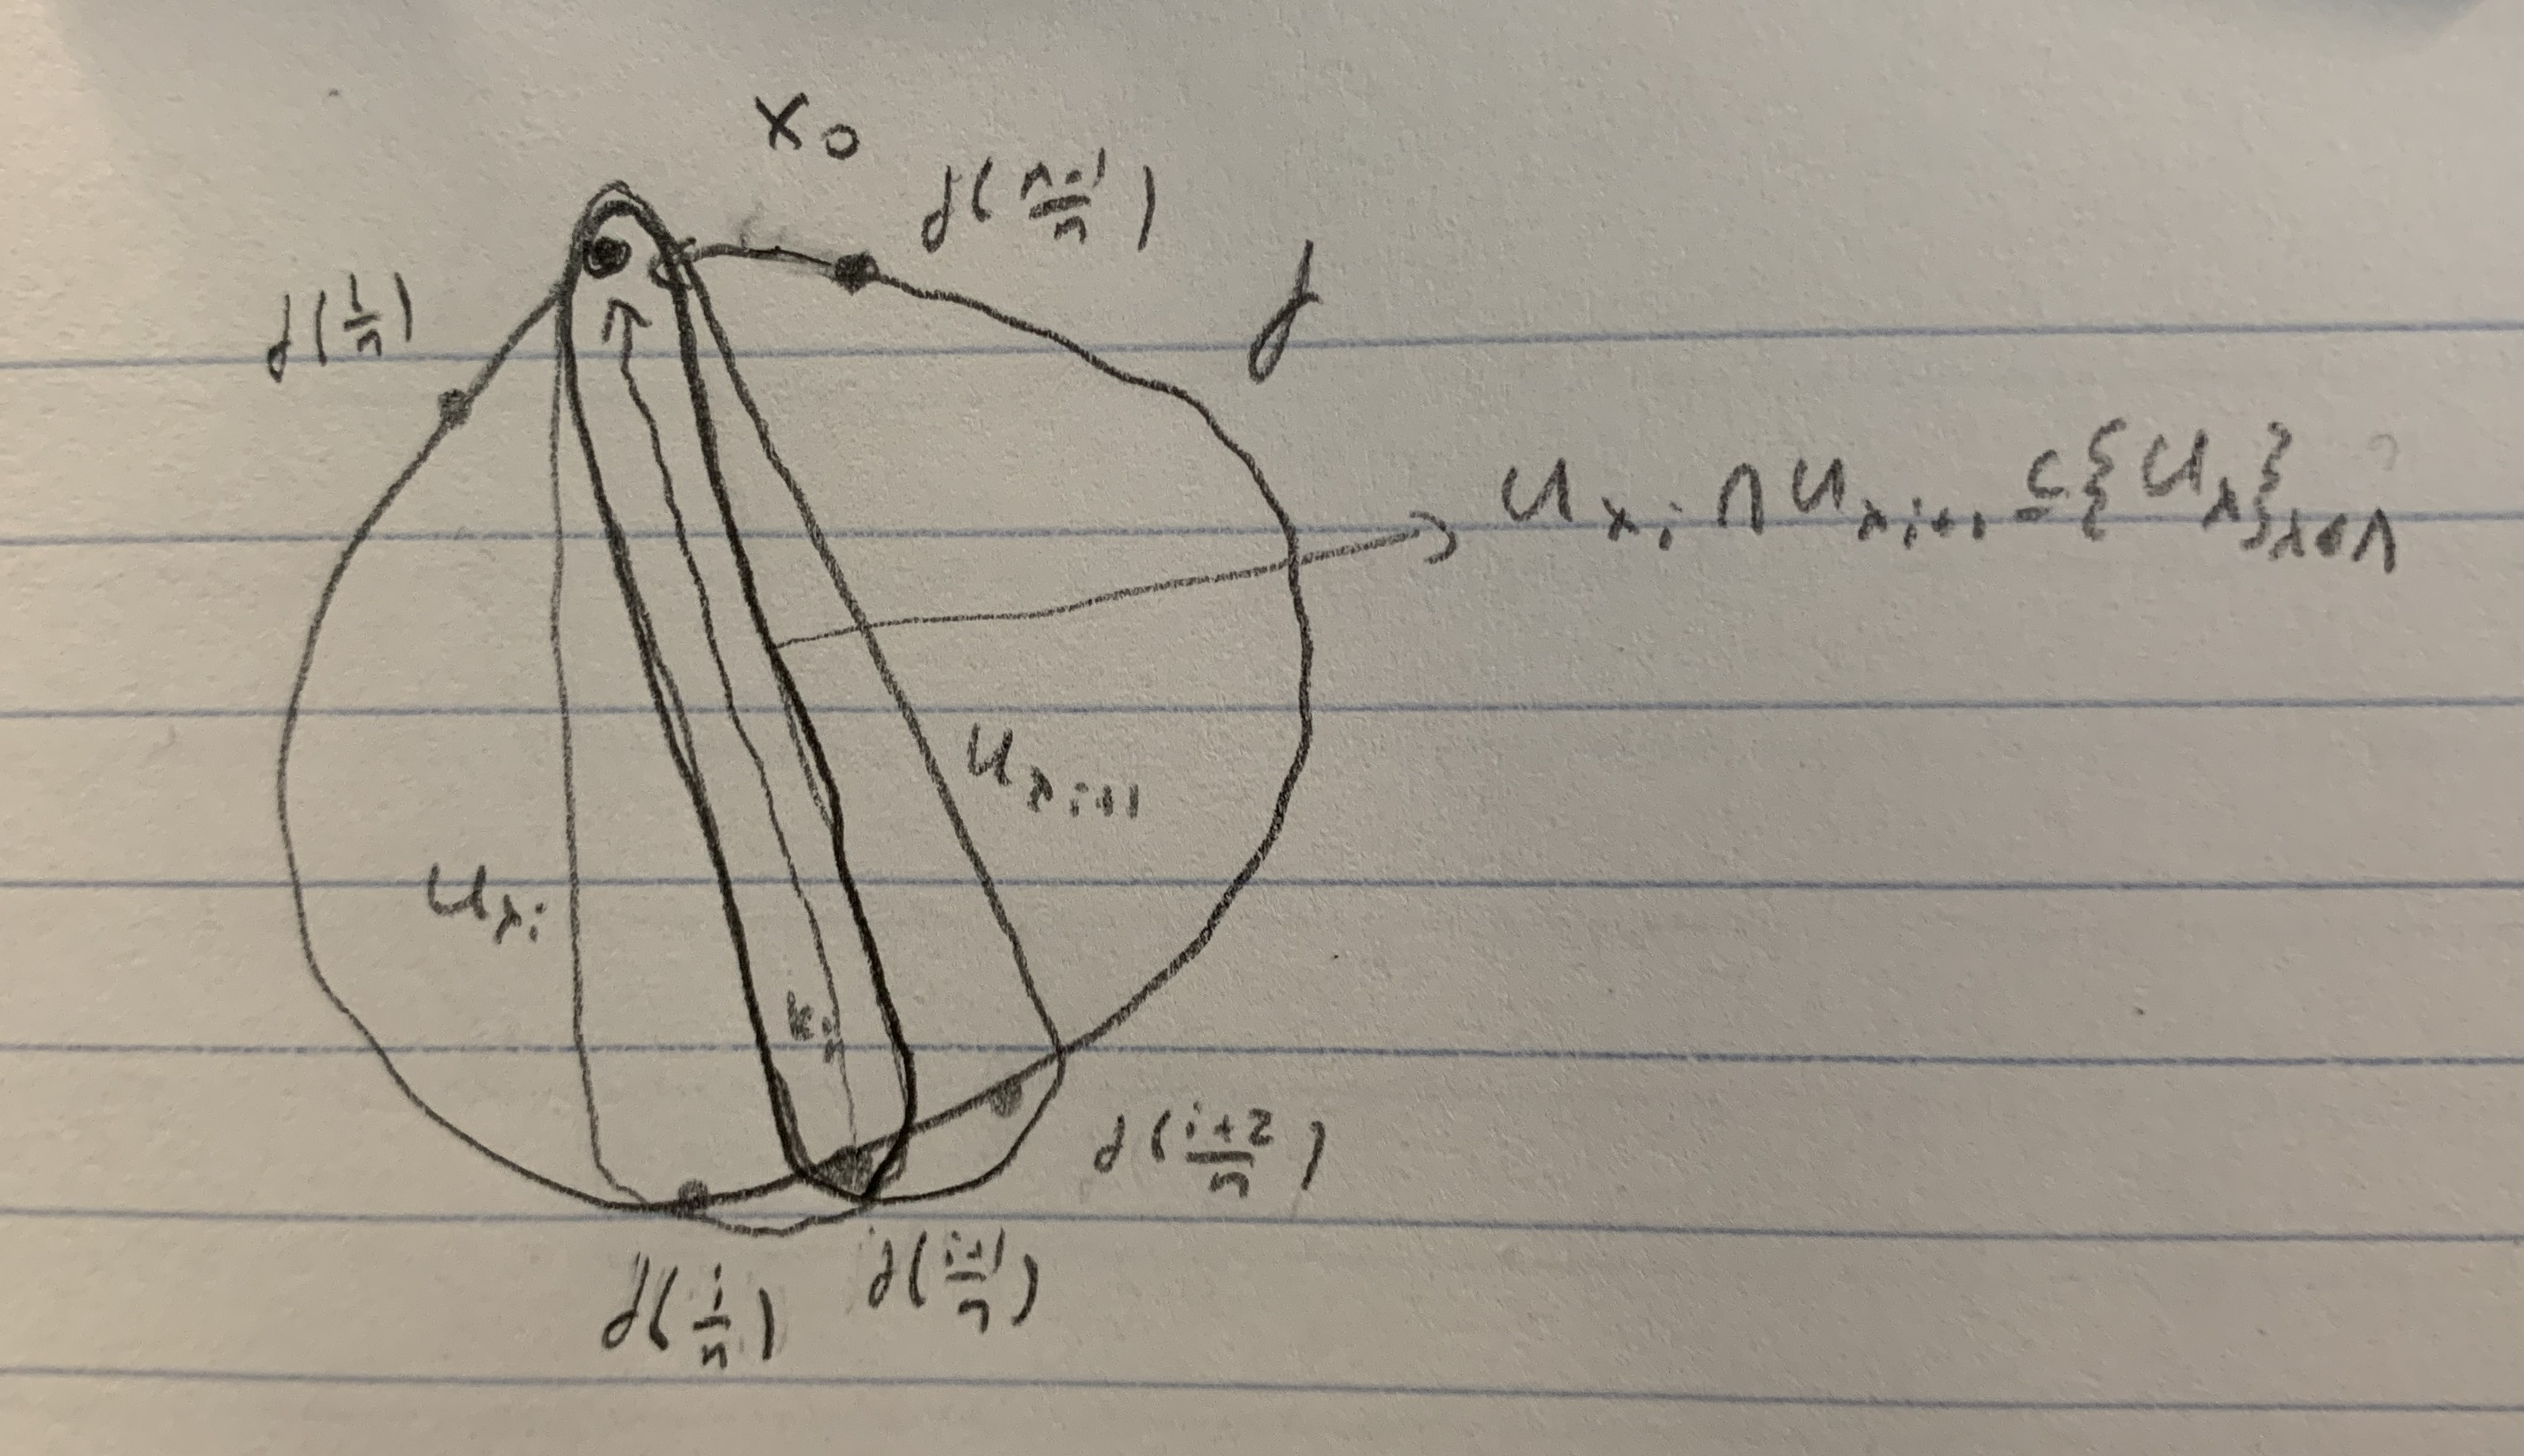
\includegraphics[width=0.7\textwidth]{img/proof-pt1.JPG}
        \end{center}
        \begin{itemize}
          \item We add the $k_i$ to put each small piece starts and ends at $x_0$,
            and so is in a fundemental group:
              \[f \sim f_1k_1\cdot k_1^{-1}f_2k_2 \cdot k_2^{-1}f_3k_3 \cdot ... \cdot k_{n-1}^{-1}f_n\]
              \[a = [f]_{\pi_1(X)} = [f_1k_1]_{\pi_1(X)} [k_1^{-1}f_2k_2]_{\pi_1(X)}
                 ... [k_{n-1}^{-1}f_n]_{\pi_1(X)}\]
            Now, $k_{i-1}f_ik_i \subseteq U_{\lambda_i}$, since $k_i \subseteq
            U_{\lambda_i}, U_{\lambda_{i+1}}$. Since $\psi_{\lambda_i}$ is the
            homomorphism induced by an inclusion map,
              \[ a = \psi_{\lambda_1}([f_1k_1]_{\pi_1(U_{\lambda_1})}) ...
                \psi_{\lambda_n}( [k_{n-1}f_n]_{\pi_1(U_{\lambda_n})})\]

        \end{itemize}
      \end{column}
    \end{columns}
  \end{frame}


\end{document}
